% !TEX root =  ../master.tex
\chapter{Anforderungsanalyse} % TODO: Das hier ist noch etwas durcheinander
\section{Abgrenzung}
\subsection{Abgrenzung des Funktionsumfangs}\label{sub:abgrenzung}
Im bereich Bildung gibt es viele Möglichkeiten, wie Hochschulen und Studenten unterstützt werdem können.
Primär gibt es hierbei 4 Ebenen, auf der Aktionen stattfinden können:
\begin{itemize}
    \item Politische Ebene\\
        Landesweite Veränderungen, die das gesamte Bildungssystem betreffen 
    \item Institutionsebene\\
        Veränderungen an der gesamten Bildungseinrichtung.
    \item Kursebene\\
        Aktionen innerhalb eines Kurses bzw. Vorlesung
    \item Individualebene\\
        Persönliche Veränderungen
\end{itemize}
Man kann ableiten, dass sich nicht alle Ebenen gleich für die zu entwickelnde Anwendung anbieten.
Auf politischer Ebene veränderungen durchzusetzen benötigen in der Regel ein aufwändiges Genehmigungsverwähren, welches wertvolle Zeit in Anspruch nehmen.
Da die Anwendung aber möglichst schnell Krisenbeeinträchtigte Studenten unterstützt werden sollen, muss diese Ebene bei der Entwicklung zunächst vernachlässigt werden.

Die Institutionsebene beschreibt das Management von Ressourcen innerhalb der Hochschule.
Besonders der Austauch und Weiterbildung zwischen Dozenten ist hierbei ein wichtiger Aspekt.
Problematisch ist aber die Identifizierung von Anforderungen aller Studienrichtungen.
So besitzen technische Studiengänge andere Bedürfnisse als wirtschaftlich orientierte Studiengänge.
Aus diesem Grund kann auch diese Ebene nicht genauer beachtet werden.

Stattdessen wird sich in dieser Arbeit auf die Entwicklung einer Anwendung mit dem Schwerpunkt auf der Kurs- und der Individualebene fokussiert.
Die Kursebene dient zur Weitergabe Lernmaterialien, die eine Vorlesung ergänzen.
Dies soll einen direkten Einfluss auf die Individualebene haben und den individuellen Studenten fördern.
Ziel ist es den Studenten beim Lernen zur unterstützen und das Verständnis der in der Vorlesung vermittelten Informationen zu fördern.  

\begin{figure}[]%FIXME:
    \begin{center}
        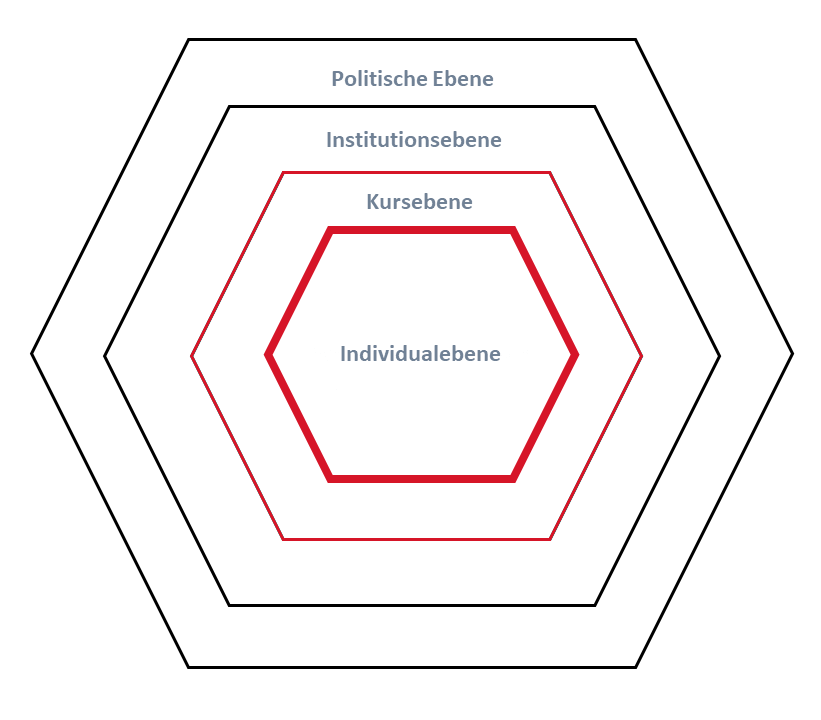
\includegraphics[width=.7\textwidth]{img/Ebenen.png}
        \caption{Aktionsebenen}
        \label{fig:ebenen}
    \end{center}
\end{figure}
%TODO: Verweis auf pptx Fr. Honal % TODO: Gibt es hier noch Quellen?

Durch diesen Fokus entfallen allerdings Vorteile, die sich durch eine größere Nutzer- und damit Datenbasis ergeben.
Besonders die Möglichkeit für Datenanalysen als Teil des Data Minings ist aufgrund des geringen Datenumfangs nicht möglich.
Gleichzeitig sind wir der Überzeugung, dass eine Auswertung des Lernfortschrittes nicht der primäre Grund für die Entwicklung einer Anwendung sein sollte, sondern der Mehrgewinn für Studenten.
Sollte sich die Anwendung für Nutzer als Vorteilhaft erweisen, kann die Anwendung ohne Probleme um Funktionalitäten aus anderen Ebenen erweitert werden.



% TODO: Können Wir vielleicht noch einen User Acceptance Test machen?

% Um eine Fortführung und Integration der anderen Ebenen in Zukunft zu ermöglichen, soll die Datenhaltung und Architektur der Anwendung so konzipiert werden, dass eine Erweiterung leicht möglich ist.

% TODO: Also bauen wir einen Export? Das wäre gut, dann können wir das schreiben. Aber da müssen wir mal schauen. Vordefinierte Auswertungen, Berechnungen wird es allerdings aufgrund der gewählten Abgrenzungen erst einmal nicht geben.
% Die vorhandenen Daten sollen im Ersten Schritt in einem auswertungstauglichen Format zur Verfügung gestellt werden.
% Die Auswertung selbst muss durch den Dozenten selbst erfolgen.

% TODO: Abgrenzung zu anderen Werkzeugen
\subsection{Abgrenzung zu anderen Anwendungen}
Im Hochschulkontext kommen bereits mehrere Systeme zum Einsatz.
Die primäre Plattform bildet \enquote{Moodle}.
Moodle ist eine Lernplattform, in dem Nutzer Kurse, Kalender, Foren und ähnliche Funktionen anbietet, die zur Steuerung und Verwaltung von Vorlesungen bietet.
Trotz des recht umfangreichen Funktionsumfangs besitzt die Anwendung aber einige Nachteile.
So berichten viele Nutzer (Studenten, Dozenten und Unternehmensbetreuer) von sehr schlechter Bedienbarkeit und Unübersichtlichkeit.
Zusätzlich weißt die Datenschutzerklärung darauf hin, dass umfangreich Daten, z.\,B. \enquote{ob und wie sie [Nutzer] in Workshops mitgewirkt haben}, gesammelt werden können.\autocites{moodleTermsOfServiceDHBW}{moodleTermsOfService}
Aus Datenschutzrechtlichen Gründen, wird aktuell die Learning Analytics Erweiterungen und Möglichkeiten der Kursmanagement und Lernplattform Moodle nicht genutzt.

Ein weiteres Werkzeug, welches von im Hochschulkontext verwendet wird ist \enquote{Dualis}.
Diese Anwendung besitzt aber nur Auskunft über Bewertungen.
Anwender können somit erste Feedback zu ihren Klausuren erhalten, sobald sie Klausuren bereits beschrieben haben.
Somit besitzen die Studenen vor der Klausur oft kein Feedback zu der von ihnen geleisteten Arbeit.

Darüber hinaus existieren Anstrengungen weitere Anwendungen umzusetzen, die aber nicht den Prototypstatus verlassen haben.
Ein Beispiel hierfür ist die MyLA-Anwendung.\autocite{mylaGithub}
Für Dozenten gibt es die Möglichkeit, Umfragen zu erstellen und mit ihren Studierenden zu teilen.
Diese haben dadurch die Chance, ihre Meinung zur Vorlesung mitzuteilen, Gelerntes zu verinnerlichen oder auch um Anmerkungen zu gestellten Fragen zu geben.
Die Plattform ermöglicht es dabei, Umfragen als Vorlage zu speichern, sodass diese in unterschiedlichen Kursen verwendet werden können und zeigt die Ergebnisse der Umfragen graphisch an.

% TODO: evasys   Dann kann man sagen, dass mehrer Anwendungen genutzt werden müssen

% TODO: Hier noch einen Satz, alle anderen Anwendungen sind Käse, und dass wir das alles super toll machen


\section{Ist-Analyse} % TODO: Ist es besser die Ist-Analyse mit den funktionalen Anforderungen zusammen zu zeihen? Ich denke schon!
Bevor die eigentliche Entwicklungs starten kann müssen die aktuellen Probleme und Verbesserungspotenziale analysiert werden.

Dozierende haben aktuell wenig Möglichkeiten zu erfahren, wie ihre Vorlesung in verschiedenen Kursen angenommen wird.
Besonders der Lernstand der Studierenden und die Stimmung innerhalb der Kurse sind nur schwer erfassbar.
Nach Aussage eines Dozenten wurde uns gesagt, dass dies besonders in Online-Vorlesungen problematisch ist.
Sofern man \enquote{nicht in fragende Gesichter schaut}, ist es ob schwer zu wissen, wann eine Fragestellung zu kompliziert ist.
Besonders durch die anonyme Maße in Online-Vorlesungen, die auch keine Kameras besitzen dies ein erhebliches Problem.
Dadurch entsteht eine Differenz, die sich in Klausuren negativ auswirken kann.
Aktuell (Dezember '20) finden zum zweiten Mal ausschließlich Online-Vorlesungen statt, sodass diese Möglichkeiten für Dozierende nochmals relevanter sein könnten.



\section{Anforderungsformulierung}

\subsection{Funktionale Anforderungen} 
Bei der Anforderungsanalyse gehen wir nach dem Motto "Von Studenten für Studenten" vor.
Wir als Studenten der DHBW können sehr gut einschätzen was uns das Studium erleichtern würde und wie wir uns in Bezug auf Klausuren und Prüfungen organisieren.
Mit einer Prozessierung und Automatisierung können Synergien genutzt werden und auch andere Kommilitonen von den für diese Veranstaltungen eingebrachten Aufwänden profitieren.

Ziel dieser Arbeit ist es eine App zu entwickeln, die Plattform unabhängig als Web-Applikation oder im Browser genutzt werden kann.
Dabei sollen sowohl Studenten als auch Dozenten einen Zugang bekommen.
Wir setzen auf eine freiwillige Teilnahme.
Die Anwendungen soll durch ihre Funktionen und die intuitive Bedienbarkeit überzeugen und nicht durch einen Nutzungszwang.

Wir konnten die folgenden funktionalen Anforderungen definieren:
\begin{itemize}
    \item Anmeldung                         \\
        Es muss eine Möglichkeit geben, wie neue Studenten und Dozenten die Anwendung nutzen können.
        In der DHBW kommen mit jedem Semester neue Studenten und neue Dozenten.
        Aus diesem Grund muss es eine Möglichkeit geben, neue Nutzer für die Nutzung der Anwendung zu authorisieren.
        Eine Anmeldung kapselt außerdem die Daten einzelner Nutzer.
    \item Kurszuweisung                     \\
        In \autoref{sub:abgrenzung} wurde bereits beschrieben, dass die Kursebene abgedeckt wird.
        Aus diesem Grund muss es eine Möglichkeit geben, Studenten zu Kursen zuzuweisen.
        Kurse sollen dabei eine logische Abgrenzung bilden, sodass Studenten nicht den Lernstoff zwischen verschiedenen Vorlesungen durcheinander bringen.
    \item TODOs                             \\
        Bisher ist es schwer einen Überblick über alle Aufgaben zu haben, die von Studenten zu erledigen sind.
        Besonders die Vielzahl an Vorlesungen, die sich in ihrem Aufbau und in der Prüfungsweise unterscheiden brauchen unterschiedliche Vorbereitungen und damit TODOs.
        TODOs können dabei optional ein Fälligkeitsdatum besitzen, welches zur besseren Organisation sollen die eingetragenen TODOs graphisch angezeigt werden.
        So entsteht ein Kalender und Kapazitätsengpässe rechtzeitig erkannt und durch Umplanen verhindert werden können.

    \item Karteikarten                      \\
        Für eine bessere Prüfungsvorbereitungen Karteikarten angelegt werden.
        Die Karteikarten sollen direkt in App gelernt werden, sodass kein zusätzlicher Aufwand für das Abschreiben der Karten notwendig ist.

    \item Prüfungsterminübersicht           \\
        In der Anwendung soll es eine Übersicht aller Klausuren und anderen Prüfungsleistungen geben.
        Momentan wird dies über einen Google Kalender gehandhabt, welcher über eine Zwischeninstanz verwaltet wird.
        In dem dies direkt in der Anwendung angegeben ist, können zusätzliche Informationen (z.\,B. zugelassene Hilfsmittel) leichter kommuniziert werden und die zeitliche Differenz wird aufgehoben.

    \item Kursübergreifende Informationen   \\
        Besitzt ein Nutzer einen Account, soll er Kurse anlegen können, zu denen er Informationen wie Datum von Prüfungen erfassen kann.
        Um zu verhindern, dass diese organisatorische Aufwand von jedem Studenten einzeln durchgeführt werden müssen soll es zusätzlich die Funktion geben, dass Dozenten einen Kurs anlegen können.
        Den Kursen können initial bereits Prüfungstermine, TODOs und Karteikarten mitgegeben werden.
        Somit entfällt die initiale Erstellung.
        Die zu einem Kurs gehörenden Informationen können von den Studierenden weiterhin nach belieben angepasst und ergänzt werden ohne dabei für die anderen eingeschriebenen Kursteilnehmer Daten zu verändern.
        Das Erstellen eines Kurses hat für den Dozenten den Vorteil, dass für diesen Kurs Daten zur Verfügung gestellt bekommt, die er zur Anpassung oder Evaluation seiner Vorlesung nutzen kann.
        Beispiele hierfür können sein Lerntypen der Studenten, Fortschritt beim Lernen der Karteikarten, etc.
    \item Rollendifferenzierung             \\
        Aus den bereits beschriebenen Anforderungen geht hervor, dass es eine Weise geben muss, wie Dozenten von Studenten unterschieden wird.
        Es soll verhindert werden, dass Studenten falsche Informationen bereitstellen können und so andere Studenten des gleichen Kurses schädigen.
        Aus diesem Grund sollen nur Dozenten Informationen bereitstellen können, die von mehreren Studenten eingesehen werden können.
\end{itemize}

% Das ist das was ich grad realistisch sehe. Wenn wir noch mehr implementiert haben, dann können wir das gerne noch erweitern

% TODO: Wo kommen die Personas hin? vor die Anforderungen? Vielleicht über die Anforderungsanalyse



\subsection{Nicht-Funktionale Anforderungen}
Neben den funktionalen Anforderungen gibt es auch einige nicht-funktionale Anforderungen, die beachtet werden müssen.
\begin{itemize}
    \item Geschwindigkeit\\
        Für Nutzer ist die Geschwindigkeit besonders wichtig.
        Lang ladende Anwendungen sind nicht nur nervig in der Benutzung, sondern könnten sich in der hier entwickelten Anwendung negativ auf den Lernfortschritt auswirken. Lange Ladezeiten lenken beispielsweise ab und demotivieren die Nutzung der Anwendung.
        Über lange Ladezeiten beschweren sich in einer Umfrage mehr als 70\%, wobei 25\% aller Nutzer bereits bei 4 Sekunden die Seite verlassen.\autocite{loadingTimes}
        Aus diesem Grund sollte die Ladezeit gering gehalten werden.
    \item Persistenter Speicher             \\
        Informationen über Kurse müssen dauerhaft gespeichert sein und jederzeit abrufbar sein.
        Besonders vor und nach Vorlesungen wird die Nutzung der Anwendung vorraussichtlich deutlich ansteigen.
        Auch bei Spitzenlast müssen stets alle Informationen abrufbar sein.
    \item Responsive Design\\
        Die Anwendung sollte auf jeden Gerät vollständig funktional sein.
        Studenten nuten häufig viele Geräte mit verschiedenen Bildschirmformaten.
        Besonders unterwegs oder in öffentlichen Verkehrsmitteln sind Mobilgeräte die primären Geräte.
        Aus diesem Grund muss sich die Anwendung dynamisch an solche Geräte anpassen.
    \item Corporate Design\\
        Die DHBW besitzt ein einheitliches Design, an der man alle DHBWs und DHBW-Anwendungen erkennt.
        Damit die Anwendung sich an die DHBW angliedert, sollte die Anwendung nahe an diesem Design sein.
        Besonders das Farbschema sollte dabei einheitlich sein. % TODO: Muss das wirklich sein, das sieht halt echt nicht gut aus. Ich mag das cosmic theme ganz gern
    \item Datenschutz\\
        Das Thema Datenschutz ist so wichtig wie nie zuvor.
        Besonders der Schutz von personenbezogenen Daten steht dabei im Vordergrund.
        Wie oben bereits festgestellt wurde besitzen Anwendungen gegenwärtig problematische Datenschutzlagen.
        Aus diesem Grund soll die entwickelte Anwendung einen hohen Wert auf den Datenschutz legen und die Verarbeitung dieser Daten auf ein Minimum reduzieren.
\end{itemize}



\subsection{Zusammenfassung}
Die gerade beschriebenen funktionalen und nicht-funktionalen Anforderungen sind noch übersichtlich und für die spätere Referenz in \autoref{tab:anforderungen} dargestellt.


\begin{table}[h]
    \centering
    \begin{tabularx}{.8\textwidth}{l|X}
        Nr.     & Beschreibung                              \\\hline
        F1      & Neue Nutzer können sich für die Nutzung anmelden                    \\
        F2      & Studenten können für Kurse eingeschrieben werden  \\
        F3      & Es können TODOs erstellt werden   \\
        F4      & Es kann mit Karteikarten gelernt werden  \\
        F5      & Prüfungstermine können eingetragen werden  \\
        F6      & Informationen können allen Studenten mitgeteilt werden  \\
        F7      & Es gibt eine Unterscheidung zwischen Studenten und Dozenten  \\
        NF1     & Anwendung lädt schnell                    \\
        NF2     & Daten jederzeit einsehbar                 \\
        NF3     & Anwendung funktioniert auf allen Geräten  \\
        NF4     & Anwendung ist am DHBW Design orientiert   \\
        NF5     & Personenbezogene Daten werden geschützt  \\
    \end{tabularx}
    \caption{Zusammengefasste Anforderungen}
    \label{tab:anforderungen}
\end{table}

% TODO: Wenn das Dashboard fertig ist, stehen da ja dann Analysen drin? Dann kann man das alles noch erweitern
% Generell Umfragen, .... alles erst reinschreiben, wenn wir das auch implementiert haben :)
